\documentclass{article}
\title{Making geological sense of `Big Data'\\in sedimentary provenance analysis}
\author{Pieter Vermeesch$^a$\footnote{corresponding author, email: {\tt p.vermeesch@ucl.ac.uk}, tel: +44 (0)20 7679 2428} and Eduardo Garzanti$^b$\\~\\
${}^a$London Geochronology Centre, University College London, United Kingdom\\
${}^b$Laboratory for Provenance Studies, Universit\`{a} di Milano-Bicocca, Italy}
\usepackage{fullpage,graphicx,natbib,amsmath,lineno}
\date{}
%\linespread{1.2}
\begin{document}
%\linenumbers

\maketitle

\begin{abstract}
Sedimentary provenance studies increasingly apply multiple chemical,
mineralogical and isotopic proxies to many samples.  The resulting
datasets are often so large (containing thousands of numerical values)
and complex (comprising multiple dimensions) that it is warranted to
use the internet-era term `Big Data' to describe them. This paper
introduces Multidimensional Scaling (MDS), Generalised Procrustes
Analysis (GPA) and Individual Differences Scaling (INDSCAL, a type of
`3-way MDS' algorithm) as simple yet powerful tools to extract
geological insights from `Big Data' in a provenance context.  Using a
dataset from the Namib Sand Sea as a test case, we show how MDS can be
used to visualise the similarities and differences between 16 fluvial
and aeolian sand samples for five different provenance proxies,
resulting in five different `configurations'.  These configurations
can be fed into a GPA algorithm, which translates, rotates, scales and
reflects them to extract a `consensus view' for all the data
considered together. Alternatively, the five proxies can be jointly
analysed by INDSCAL, which fits the data with not one but two sets of
coordinates: the `group configuration', which strongly resembles the
graphical output produced by GPA, and the `source weights', which can
be used to attach geological meaning to the group configuration. For
the Namib study, the three methods paint a detailed and
self-consistent picture of a sediment routing system in which sand
composition is determined by the combination of provenance and
hydraulic sorting effects.
\end{abstract}
\begin{center}
\emph{keywords: provenance -- statistics -- sediments -- U-Pb -- zircon -- heavy minerals}
\end{center}
\section{Introduction}
\label{sec:intro}

Some 65\% of Earth's surface is covered by siliclastic sediments and
sedimentary rocks. Unravelling the provenance of these materials is of
key importance to understanding modern sedimentary environments and
their ancient counterparts, with important applications for
geomorphology, paleotectonic and paleogeographic reconstructions,
hydrocarbon exploration and reservoir characterization, and even
forensic science \citep[e.g.,][]{pye2007, vermeesch2010b,
  garzanti2012, garzanti2014b, garzanti2014c, stevens2013, nie2014,
  scott2014}.  Over the years, thousands of studies have used a
plethora of chemical, mineralogical and isotopic indicators to trace
sedimentary provenance. The complexity of the resulting datasets can
be organised on a number of hierarchical levels:

\begin{enumerate}

\item{A single sample}

Siliclastic sediments are made of grains, and on the most basic level,
geological provenance analysis extracts certain properties from these
grains. These properties can either be categorical (e.g, mineralogy)
or continuous (e.g., age). In rare cases, analysing just a single
grain can already yield important insight into the provenance of a
sediment. For example, a single grain of alluvial diamond confirms the
existence of kimberlitic lithologies in the hinterland. In general,
however, provenance studies require not just one but many grains to be
analysed. The provenance information contained in a representative
collection of grains can be visualised with graphical aids such as
histograms, pie charts or kernel density estimates
\citep{vermeesch2012b}.

\item{Multiple samples}

Subjective comparison of detrital zircon U-Pb age distributions or
heavy mineral compositions reveals the salient similarities and
differences between two samples. Things become more complicated when
more than two samples need to be compared simultaneously.  For
example, a dataset comprising n = 10 age distributions presents the
observer with n(n-1)/2 = 45 pairwise comparisons. If n = 100, this
increases quadratically to 4,950 pairwise comparisons, which is
clearly too much for the human brain to process. Multi-Dimensional
Scaling (MDS) is a technique aimed to simplify this exercise (Section
\ref{sec:MDS}). Originating from the field of psychology, the method
is commonly used in ecology \citep{kenkel1986} and palaeontology
\citep[e.g.,][]{dunkley2008, schneider2011}. MDS was introduced to the
provenance community by \citet{vermeesch2013}, and has instantly
proved its value for the interpretation of large datasets
\citep[e.g.,][]{stevens2013, nie2014}.

\item{Multiple methods}

Several provenance methods are in use today which can be broadly
categorised into two groups. Each of these tells a different part of
the provenance story:

\begin{enumerate}
\item{\bf Multi-mineral} techniques such as heavy mineral analysis and
  bulk geochemistry provide arguably the richest source of provenance
  information, but are susceptible to hydraulic sorting effects during
  deposition as well as chemical dissolution by diagenesis and
  weathering \citep{garzanti2009, ando2012}.  These effects obscure
  the provenance signal and can be hard to correct.

\item{\bf Single mineral} techniques such as detrital zircon U-Pb
  geochronology are less sensitive to hydraulic sorting effects and,
  in the case of zircon, scarcely affected by secondary processes as
  well. However, zircon is `blind' to sediment sources such as mafic
  volcanic rocks and carbonates. Furthermore, the robustness of zircon
  comes at a price, as it is difficult to account for the effect of
  sediment recycling \citep{garzanti2013}.
\end{enumerate}

Great benefits arise when these two types of methods are used in
tandem. A string of recent studies combining conventional bulk and
heavy mineral petrography techniques with detrital geochronology have
shown that this provides a very powerful way to trace provenance
\citep[e.g,][]{stevens2013, garzanti2012, garzanti2014b,
  garzanti2014c}.  Combining multiple methods adds another level of
complexity which requires an additional layer of statistical
simplification.  The datasets resulting from these multi-sample,
multi-method studies are so large and complex that it is warranted to
use the internet-era term `Big Data' to describe them.  This paper
introduces Procrustes analysis (Section \ref{sec:procrustes}) and
3-way MDS (Section \ref{sec:indscal}) as valuable tools to help make
geological sense of `Big Data'. These methods will be applied to a
large dataset from the Namib Sand Sea, which combines 16 samples
analysed by 5 different methods (Section \ref{sec:data}). Although the
use of some mathematical equations was inevitable in this paper, we
have made the text as accessible as possible by reducing the
algorithms to their simplest possible form. The formulas given in
Sections \ref{sec:MDS}-\ref{sec:indscal} should therefore be
considered as conceptual summaries rather than practical recipes, with
further implementational details deferred to the Appendices.

\end{enumerate}

\section{The Namib dataset}
\label{sec:data}

The statistical methods introduced in this paper will be illustrated
with a large dataset from Namibia. The dataset comprises fourteen
aeolian samples from the Namib Sand Sea and two fluvial samples from
the Orange River (Figure \ref{fig:data}).  These samples were analysed
using five different analytical methods:

\begin{enumerate}
\item{Geochronology:} $\sim$100 zircon U-Pb ages were obtained per
  sample by LA-ICP-MS. For samples N1-N13, this was done using methods
  described by \citet{vermeesch2010b}.  N14, T8 and T13 are new
  samples which were analysed at the London Geochronology Centre using
  an Agilent 7700x ICP-MS coupled to a New Wave NWR193 excimer laser
  with standard two volume ablation cell.
\item{Heavy minerals:} a full description of samples N1-N14 was given
  by \citet{garzanti2012}. Samples T8 and T13 were reported (as
  samples S4328 and S4332) by \citet{garzanti2014b,garzanti2014c}.
\item{Bulk petrography:} is also taken from
  \citet{garzanti2012,garzanti2014b,garzanti2014c}.
\item{Major element composition:} 10 major elements were measured by
  acid dissolution (Aqua Regia) ICP-ES at AcmeLabs Inc. in Vancouver,
  Canada (protocol 4A/B).
\item{Trace element composition: 27 trace elements were measured by
  acid dissolution (Aqua Regia) ICP-ES and ICP-MS at AcmeLabs
  (protocol 4A/B).}
\end{enumerate}

The complete dataset is available as an Online Supplement in a tabular
form that can be imported into the software discussed later in this
paper.  Taken altogether, the entire dataset contains 16,125 physical
measurements covering a variety of ordinal and compositional
spaces. This is a prime example of `Big Data' in a provenance
context. A lot can be learned by a simple qualitative analysis of the
measurements. For example, the zircon age distributions reveal
prominent peaks at $\sim$600 and $\sim$1,000 Ma, consistent with a
hinterland affected by Damara and Namaqua orogenesis, while the
widespread occurrence of pyroxene and basaltic rock fragments
indicates the existence of a volcanic sediment source
\citep{garzanti2012, garzanti2014b}. But it is difficult to go beyond
these general observations without statistical assistance because
there is simply `too much' data. In the following sections, we will
follow the hierarchical organisation of Section \ref{sec:intro} to
gain a better understanding of the multivariate dataset in different
steps. First, we will integrate the different age distributions and
compositions into five MDS maps (Section \ref{sec:MDS}). Then, we will
integrate these MDS maps into a single `Procrustes analysis' (Section
\ref{sec:procrustes}).  Finally, we will jointly analyse the five
datasets using `3-way MDS' to gain further insight into the sediment
routing system (Section \ref{sec:indscal}).

\begin{figure}[!ht]
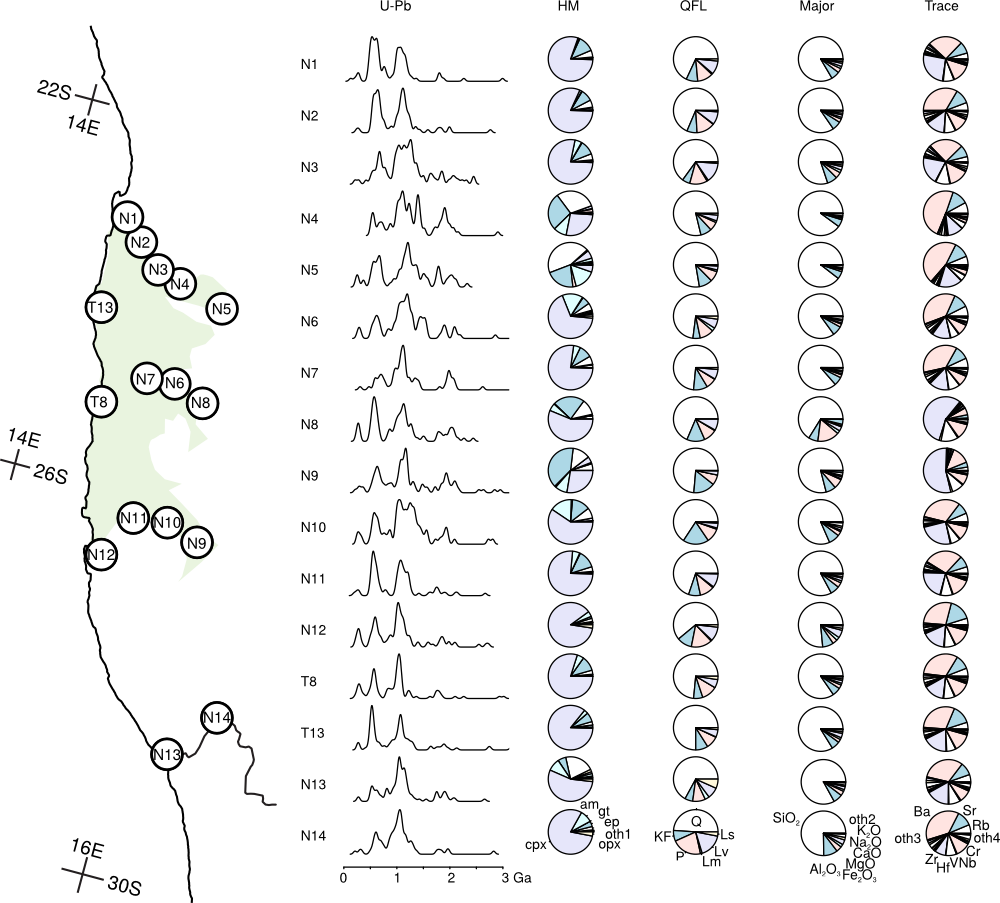
\includegraphics[width=\textwidth]{NamData.png}
\caption{The Namib dataset comprises of 1,533 detrital zircon U-Pb
  ages \citep[shown as kernel density estimates with a bandwidth of 30
    Ma,][]{vermeesch2012b}, 3,600 heavy mineral counts (`HM'), 6,400
  petrographic point counts (`QFL'), and chemical concentration
  measurements for 10 major and 27 trace elements.  `opx' =
  orthopyroxene, `cpx' = clinopyroxene, `am' = amphibole, `gt' =
  garnet, `ep' = epidote, `oth1' = zircon + tourmaline + rutile +
  Ti-oxides + sphene + apatite + staurolite; `Q' = quartz, `KF' =
  K-feldspar, `P' = plagioclase, `Lm', `Lv' and `Ls' are lithic
  fragments of metamorphic, volcanic and sedimentary origin,
  respectively; `oth2' = TiO$_2$ + P$_2$O$_5$ + MnO; `oth3' = Sc + Y +
  La + Ce + Pr + Nd + Sm + Gd + Dy + Er + Yb + Th + U, and `oth4' = Cr
  + Co + Ni + Cu + Zn + Ga + Pb. This figure makes the point that an
  objective interpretation of a large database like this is impossible
  without the help of statistical aids.}
\label{fig:data}
\end{figure}

\section{Multidimensional Scaling}
\label{sec:MDS}

The Namib study contains 16 samples, which can be visualised as kernel
density estimates (for the U-Pb data) or pie charts/histograms (for
the compositional datasets). For each of the five provenance proxies,
we have 16$\times$15/2 = 120 pairwise comparisons, which is clearly
too much to handle for an unaided human observer (Figure
\ref{fig:data}).  Multidimensional Scaling (MDS) is a technique aimed
to simplify the interpretation of such large datasets by producing a
simple two-dimensional map in which `similar' samples plot close
together and `dissimilar' samples plot far apart. The technique is
rooted in the field of psychology, in which human observers are
frequently asked to make a subjective assessment of the dissimilarity
between `stimuli' such as shapes, sounds, flavours etc. A classic
example of this is the colour-vision experiment of \citet{helm1964},
which recorded the perceived differences between 10 colours by a human
observer, resulting in a 9$\times$9 dissimilarity matrix. Let
$\delta_{i,j}$ be the `dissimilarity' between two colours i and j
(`red' and `blue', say). Then MDS aims to find a monotone `disparity
transformation' f

\begin{equation}
f(\delta_{ij}) = \delta'_{ij}
\label{eq:f}
\end{equation}

and a configuration\footnote{In this paper we will only consider
  two-dimensional solutions, which simplfies the notation and
  interpretation. It is easy to generalise the equations to more than
  two dimensions.} X

\begin{equation}
X = \left[
\begin{array}{cccccccc}
x_1 & x_2 & \cdots & x_i & \cdots & x_j \cdots & x_n\\
y_1 & y_2 & \cdots & y_i & \cdots & y_j \cdots & y_n
\end{array}
\right]
\label{eq:X}
\end{equation}

so as to minimise the (`raw') stress S

\begin{equation}
S = \sum\limits_{i<j} \left[\delta'_{ij} - \sqrt{(x_i-x_j)^2+(y_i-y_j)^2}\right]^2
\label{eq:stress}
\end{equation}

The (x,y)-coordinates resulting from Equation \ref{eq:X} can be
plotted as a map which, in the case of the \citet{helm1964} dataset,
reveals the well-known colour circle (Figure \ref{fig:2way}a). Exactly
the same principle can be used for geological data with, of course,
dissimilarities not based on subjective perceptions but analytical
data.  There is a rich literature documenting ways to quantify the
dissimilarity between petrographic or geochemical datasets. Further
details about this are provided in Appendix A.\\

Applying these methods to the Namib dataset, we can convert the raw
input data (Figure \ref{fig:data}) into five dissimilarity
matrices. For the purpose of this exercise, we have used the
Kolmogorov-Smirnov statistic for the U-Pb data, the Bray-Curtis
dissimilarity for the heavy mineral and bulk petrography data, and the
Aitchison distance for the major and trace element compositions (see
Appendix A for a justification of these choices). Each of the
resulting dissimilarity matrices can then be fed into an MDS algorithm
to produce five configurations (Figure \ref{fig:2way}).  Note that,
because the Bray-Curtis dissimilarity does not fulfil the triangle
inequality, the petrographic and heavy mineral datasets cannot be
analysed by means of classical MDS \citep{vermeesch2013}. The MDS maps
of Figure \ref{fig:2way} were therefore constructed using a nonmetric
algorithm \citep[see][for further details]{kruskal1978, borg2005,
  vermeesch2013}. It is important to note that nonmetric MDS merely
aims to reproduce the `rank order' of the input data, rather than the
actual dissimilarities themselves \citep{kruskal1964,
  borg2005}. Bearing this in mind, the five MDS maps representing the
Namib dataset reveal some clear trends in the data.\\

A first observation is that the coastal samples (N1, N2, N11, N12, T8
and T13) plot close together in all five MDS maps, with the
easternmost samples (N4, N5, N8 and N9) plotting elsewhere. Second,
the Orange River samples (N13 and N14) tend to plot closer to the
coastal samples than to the inland samples. And third, within the
eastern group, the northern samples (N4 and N5) are generally found in
a different direction from the southern samples (N8 and N9), relative
to the coastal group. But in addition to these commonalities, there
also exist notable differences between the five maps. Specific
examples of this are the odd position of N14 in the bulk petrography
configuration (Figure \ref{fig:2way}d), the different orientation of
the major and trace element configurations (Figures \ref{fig:2way}e
and \ref{fig:2way}f) and countless other minor differences in the
absolute and relative inter-sample distances.  Also note that not all
five datasets fit their respective MDS configuration equally well. A
`goodness of fit' measure called `Stress-1' can be obtained by
normalising the `raw' stress (Equation \ref{eq:stress}) to the sum of
the squared fitted distances \citep{kruskal1964, kruskal1978}.  The
resulting Stress-1 values range from 0.02 to 0.07, indicating
`excellent' fits to some and `fair' fits to other datasets (Figure
\ref{fig:2way}b-f). The five MDS maps, then, present us with a
multi-comparison problem similar to the one presented by Figure
\ref{fig:data}, with the only difference being that it does not
involve multiple KDEs or pie charts, but multiple MDS maps. Making
this multi-sample comparison more objective requires an additional
layer of statistical simplification, in which all the data are pooled
to produce a `consensus' view.

\begin{figure}[!ht]
\centering
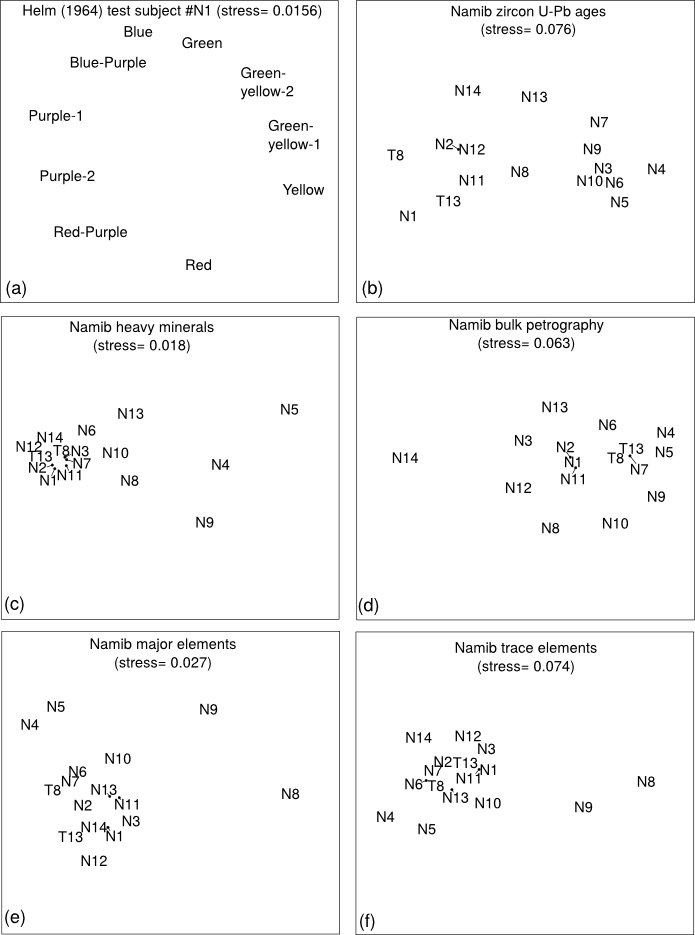
\includegraphics[height=.7\textheight]{2way3.png}
\caption{Nonmetric (2-way) MDS analyses of (a) \citet{helm1964}'s
  colour-vision data (for a single observer, `N1') and (b)-(f) the
  five Namib datasets. The `stress' values indicate `excellent'
  ($<0.025$) to `fair' ($<$0.1) fits \citep{kruskal1978,
    vermeesch2013}. Axes are plotted on a one-to-one scale with
  omitted labels to reflect the fact that non-metric MDS aims to
  preserve the ranks rather than the values of the
  dissimilarities. The MDS maps for the Namib dataset all paint a
  consistent picture in which (i) the coastal dune and Orange river
  samples (N1, N2, N11, N12, T8 and T13) plot close together and the
  inland samples (N4, N5, N8 and N9) plot elsewhere; and (ii) the
  northeastern samples (N4 and N5) are generally found in a different
  direction from the southeastern samples (N8 and N9), relative to the
  coastal group. However, there are also some distinct differences
  between the five configurations. The Procrustes and 3-way MDS
  analysis presented in Figures \ref{fig:procrustes} and
  \ref{fig:3-way} make an abstraction of these differences.}
\label{fig:2way}
\end{figure}

\section{Procrustes analysis}
\label{sec:procrustes}

According to Greek mythology, Procrustes was an inn keeper who managed
to fit all travellers to a single bed, regardless of their size or
length, by stretching or amputation. Similarly, in a statistical
context, a Procrustes arrangement can be found that resembles each of
several MDS maps by a combination of stretching, translation,
reflection and rotation. In mathematical terms, Generalised Procrustes
Analysis \citep[GPA,][]{gower1975, gower2004, borg2005} proceeds in a
similar manner to the method laid out for MDS in Section
\ref{sec:MDS}. Given $K$ sets of two-dimensional MDS configurations
$X_k$ (for 1 $\leq k \leq K$)

\begin{equation}
X_k = \left[
\begin{array}{cccccc}
x_{1k} & x_{2k} & \cdots & x_{ik} & \cdots & x_{nk}\\
y_{1k} & y_{2k} & \cdots & y_{ik} & \cdots & y_{nk}
\end{array}
\right]
\label{eq:Xk}
\end{equation}

GPA aims to find a transformation g constituting of a combination of
scale factors $s_k$, orthonormal transformation matrices $T_k$ and
translation matrices $t_k$ \citep{borg2005}:

\begin{equation}
g(X_k) = s_k X_k T_k + t_k = X'_k = \left[
\begin{array}{cccccc}
x'_{1k} & x'_{2k} & \cdots & x'_{ik} & \cdots & x'_{nk}\\
y'_{1k} & y'_{2k} & \cdots & y'_{ik} & \cdots & y'_{nk}
\end{array}
\right]
\label{eq:g}
\end{equation}

and a `group configuration' $\bar{X}$

\begin{equation}
\bar{X} = \left[
\begin{array}{cccccccc}
\bar{x}_{1} & \bar{x}_{2} & \cdots & \bar{x}_{i} & \cdots & \bar{x}_{j} & \cdots & \bar{x}_{n}\\
\bar{y}_{1} & \bar{y}_{2} & \cdots & \bar{y}_{i} & \cdots & \bar{y}_{j} & \cdots & \bar{y}_{n}
\end{array}
\right]
\label{eq:Xbar}
\end{equation}

so as to minimise the least squares misfit SS:

\begin{equation}
SS = \sum\limits_{k=1}^{K} \sum\limits_{i=1}^{n} (x'_{ik}-\bar{x}_{i})^2 + (y'_{ik}-\bar{y}_{i})^2
\label{eq:procrustes}
\end{equation}

Applying this method to the five (i.e., K=5) Namib MDS maps of Figure
\ref{fig:2way} produces a Procrustes map (Figure \ref{fig:procrustes})
confirming the salient points raised in Section \ref{sec:MDS}.  The
GPA analysis shows the dichotomy between the coastal and eastern
sands, as well as the similarity of the coastal sands with the Orange
River, and it does so more clearly than any of the five original MDS
maps (Figure \ref{fig:2way}). It also emphasises the significance of
the differences between the northeastern and southeastern samples,
which plot at right angles from each other relative to the coastal
samples. The GPA map, then, paints a detailed picture of the sediment
routing system in the Namib Sand Sea, which would have been difficult
to obtain from a simple visual inspection of the raw data. However,
GPA weighs all five MDS configurations equally and does not readily
take into account the significant differences in `goodness of fit'
(`Stress-1, Section \ref{sec:MDS}) between them.  Also, although the
trends and groupings among samples are clear from the GPA map, the
underlying reasons for these features are not. The next section
introduces a method aiming to solve this problem and thus yields
additional insight into the sediment routing system of Namibia.

\begin{figure}[!ht]
\centering
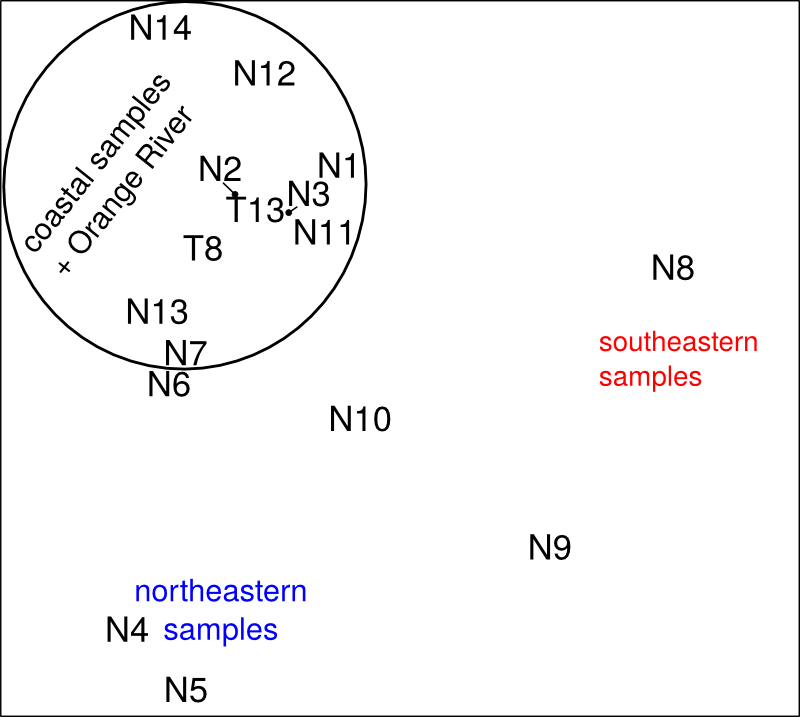
\includegraphics[width=.6\textwidth]{procrustes3.png}
\caption{Generalised Procrustes Analysis (GPA) of the Namib dataset,
  pooling together all five MDS maps of Figure \ref{fig:2way} into a
  single `average' configuration. This confirms the strong
  similarities between sand samples collected along the Atlantic coast
  (N1, N2, N11, N12, T8, T13) and the Orange River (N13 and N14) as
  opposed to samples collected further inland (N4 through N10).}
\label{fig:procrustes}
\end{figure}

\section{3-way MDS}
\label{sec:indscal}

As we saw in Section \ref{sec:procrustes}, Procrustes analysis is a
two-step process. First, the various datasets are analysed by
MDS. Then, the resulting MDS configurations are amalgamated into a
single Procrustes map. The question then arises whether it is possible
to skip the first step and go straight from the input data to a `group
configuration'.  Such methods exist under the umbrella of `3-way MDS'.
In this paper, we will discuss the oldest and still most widely used
technique of this kind, which is known as INdividual Differences
SCALing \citep[INDSCAL,][]{carroll1970}. The method is formulated as a
natural extension of the basic MDS model outlined in Section
\ref{sec:MDS}.  Given K dissimilarity matrices $\delta_{ij,k}$ ($1
\leq i,j \leq n$ and $1 \leq k \leq K$), INDSCAL aims to find K
disparity transformations $f_k$

\begin{equation}
\delta'_{ij,k} = f_k(\delta_{ij,k}) \mbox{ (with }
\sum_{i<j}\delta'^{2}_{ij,k} \mbox{ = constant } \forall~k \mbox{),}
\label{eq:fk}
\end{equation}

a group configuration $\bar{X}$ (defined as in Equation
\ref{eq:Xbar}), and a set of dimension weights W

\begin{equation}
W = \left[
\begin{array}{cccccc}
w_{x1} & w_{x2} & \cdots & w_{xk} & \cdots & w_{xK}\\
w_{y1} & w_{y2} & \cdots & w_{yk} & \cdots & w_{yK}
\end{array}
\right]
\label{eq:W}
\end{equation}

so as to minimise a modified stress parameter $S'$

\begin{equation}
S' = \sum\limits_{k=1}^{K} \sum\limits_{i<j} 
\left[\delta'_{ij,k} - \sqrt{w_{xk}(x_i-x_j)^2 + w_{yk}(y_i-y_j)^2}\right]^2
\label{eq:stress'}
\end{equation}

To illustrate the application of INDSCAL to real data, it is
instructive to revisit the colour-vision example of Section
\ref{sec:MDS}.  In addition to test subject `N1' shown in Figure
\ref{fig:2way}a, the study by \citet{helm1964} involved thirteen more
participants. Each of these people produced one (or two, for subjects
N6 and CD2) dissimilarity matrix(es), resulting in a total of sixteen
MDS maps, which could in principle be subjected to a Procrustes
analysis (Section \ref{sec:procrustes}). Alternatively, the sixteen
dissimilarity matrices can also be fed into the INDSCAL algorithm. The
resulting `group configuration' ($\bar{X}$) is a map that fits the
perceived differences of all fourteen observers by stretching and
shrinking (but not rotating) in the x- and y-direction (Figure
\ref{fig:3-way}.a).  The degree of stretching or shrinking associated
with each observer is given by the `source weights' (W), which can be
plotted as a second piece of graphical output (Figure
\ref{fig:3-way}.b).  For the colour-vision experiment, the group
configuration shows the familiar colour circle, and the source weights
express the degree to which this colour circle is distorted in the
perception of the colour deficient test subjects (prefix `CD')
relative to those subjects with normal colour vision (prefix `N'). The
latter all plot together in the northwest quadrant of the diagram,
whereas the former plot in the southeast quadrant. Multiplying the x-y
coordinates of the group configuration with the respective dimensions
of the source weights yields sixteen `private spaces', which are
approximate MDS maps for each test subject. For the colour deficient
subjects, these private spaces will have an oblate shape, emphasising
the reduced sensitivity of the colour deficient test subjects to the
red-green colour axis relative to the blue-yellow axis. In summary,
whereas an ordinary MDS configuration can be rotated by an arbitrary
angle without loss of information, this is not the case for an INDSCAL
group configuration. The principal axes of the latter generally have
an interpretive meaning, which is one of the most appealing aspects of
the method \citep{arabie1987, borg2005}.\\

The five datasets of the Namibian study can be analysed in exactly the
same manner as \citet{helm1964}'s colour data, producing the same two
pieces of graphical output as before. The resulting `group
configuration' (Figure \ref{fig:3-way}c) looks remarkably similar to
the GPA map of Figure \ref{fig:procrustes}. It shows the same
separation between samples collected from the eastern and western
parts of the desert, and the same 90$^\circ$ angle between the
northeastern and southeastern sampling locations. But whereas the GPA
map did not offer any explanation for these observations, the source
weights of the INDSCAL analysis do provide some important clues
(Figure \ref{fig:3-way}d). The provenance proxies based on the
analysis of bulk materials (chemistry and petrography) attach stronger
weights to the horizontal dimension. The proxies based on density
separates (U-Pb ages and heavy minerals), on other hand, weigh the
vertical dimension more heavily.  Because the former proxies are more
sensitive to hydraulic sorting effects and comparatively less
sensitive to provenance than the latter proxies (see Section
\ref{sec:intro}), this observation leads to the interpretation that
hydraulic sorting (predominantly) separates samples along the
x-dimension, whereas the provenance signal (predominantly) separates
samples along the y-dimension.

\begin{figure}[!ht]
\centering
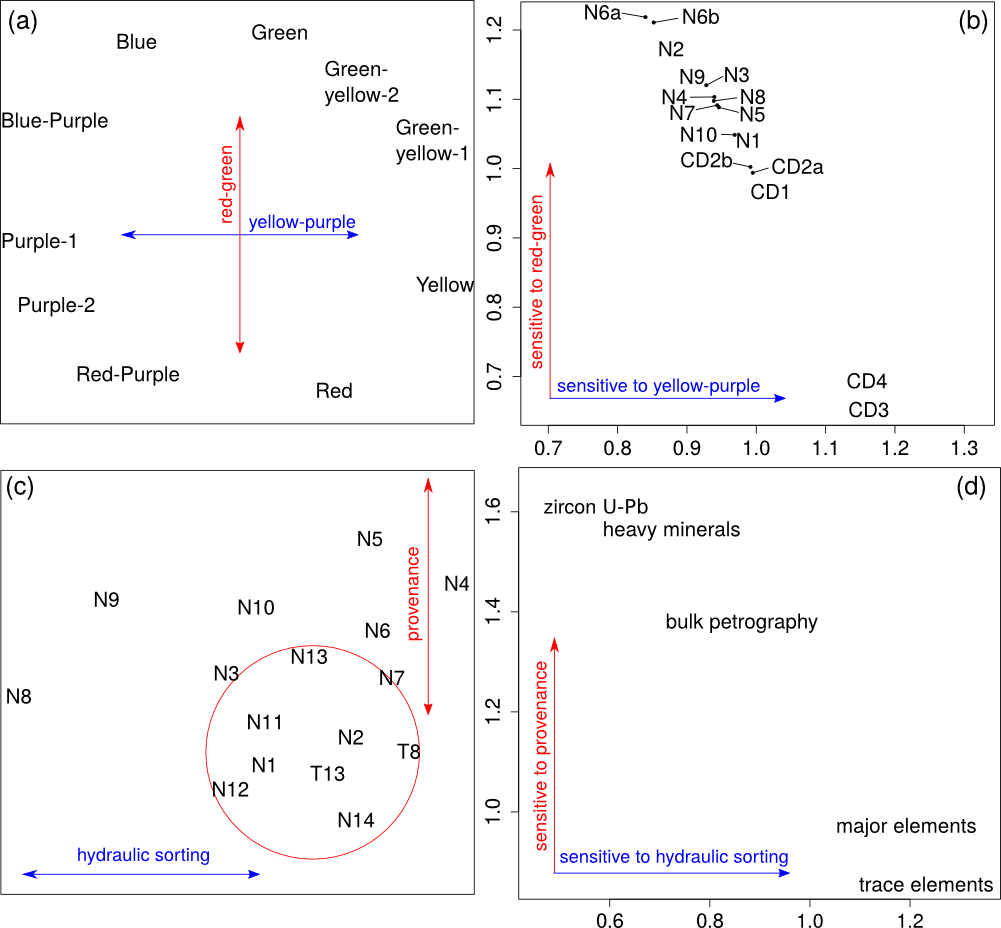
\includegraphics[width=\textwidth]{3-way3.png}
\caption{3-way MDS analysis of the colour-vision experiment by
  \citet[][(a)-(b)]{helm1964} and the Namib dataset [(c)-(d)].  The
  left panels [(a) and (c)] show the `group configurations', whereas
  the right panels [(b) and (e)] show the `source weights'.  For the
  Namib dataset, the former shows essentially the same picture as the
  Procrustes analysis (Figure \ref{fig:procrustes}). The map of
  `source weights' (d) shows the degree of importance each of the five
  proxies attach to the horizontal and vertical dimension of the group
  configuration. An intuitive interpretation of these two dimensions
  suggests that the y-axis shows the provenance signal (which
  dominates the proxies based on density separates, see Section
  \ref{sec:intro}), whereas the hydraulic sorting effect dominates the
  x-axis (and the bulk analysis proxies).}
\label{fig:3-way}
\end{figure}

\section{Discussion, caveats and conclusions}
\label{sec:discussion}

Until recently, large multi-proxy provenance studies like the Namib
case study presented in this paper were prohibitively expensive and
time consuming.  However, continued technological advances in mass
spectrometry \citep{frei2009} and petrography/geochemistry
\citep{allen2012} promise to change this picture.  In anticipation of
the impending flood of provenance data resulting from these advances,
this paper borrowed some simple yet powerful `data mining' techniques
from other scientific disciplines, which help to make geological sense
of complex datasets.  Some readers will be familiar with Principal
Components Analysis (PCA), which is a dimension-reducing procedure
that is commonly used to interpret geochemical, petrographic and other
compositional data \citep{aitchison1983,
  vermeesch2013}. Multidimensional Scaling is a flexible and powerful
superset of PCA which allows geologists to extend PCA-like
interpretation to isotopic data such as U-Pb ages
\citep{vermeesch2013}. Generalised Procrustes Analysis and Individual
Differences Scaling are higher order supersets of MDS which can be
used to integrate multiple proxies in a single comprehensive
analysis.\\

The application to the Namib Sand Sea has yielded results that are
broadly consistent with previous interpretations by visual inspection
of the age distributions, petrographic diagrams etc. The statistical
tools presented in this paper offer two key advantages over the
traditional approach.  First, they are far more objective and easy to
use. Expert knowledge of mineralogy, petrography and isotope
geochemistry, while still desirable, becomes less crucial because the
statistical tools automatically extract geologically meaningful
differences between the datasets.  Second, the methods introduced in
this paper provide a way to compare datasets of very different nature
in a common framework.  Thus the new approach to data interpretation
makes it much easier to combine petrographic and isotopic provenance
proxies.\\

Despite the intuitive appeal of INDSCAL and its apparent success in
the Namib study, it is important to mention a few caveats. Whereas the
group configuration is quite robust (as exemplified by the similarity
of Figures \ref{fig:procrustes} and \ref{fig:3-way}d), the same cannot
be said about the source weights.  Consider, for example, the INDSCAL
analysis of the Namib data, which used a combination of
Kolmogorov-Smirnov (for the U-Pb data), Bray-Curtis (for the
mineralogical data) and Aitchison (for the bulk chemistry)
measures. Replacing the Kolmogorov-Smirnov statistic with
\citep{sircombe2004a}'s L2-norm, say, results in a similar group
configuration but in significantly different source weights with a
less clear interpretation (although the bulk and density separated
proxies still plot in opposite corners). The instability of the source
weights may easily lead to over-interpretation, causing some
\citep[e.g.,][]{borg2005} to recommend abandoning INDSCAL in favour of
GPA or similar techniques.\\

Thanks to the widespread acceptance of MDS, GPA and INDSCAL in other
fields of science, several software options are available (see
Appendix B for details). These tools can be combined with other types
of inferential techniques such as cluster analysis, regression,
bootstrapping etc. This paper barely scratches the surface of the vast
field of MDS-related research. We refer the user to the reference
works by \citet{arabie1987, borg2005, borg2012, gower2004} for further
details and ideas and hope that our paper will encourage others to
explore these extension in order to address a new class of geological
problems.

\section*{Acknowledgments}

We would like to thank Ingwer Borg, Jan de Leeuw, Patrick Mair,
Patrick Groenen, Christian Hennig and two anonymous reviewers for feedback
and statistical advice. This research was funded by NERC grant 
\#NE/1009248/1 and ERC grant 259505 (`KArSD').

\section*{Appendix A: dissimilarity measures}

This section provides a few examples of dissimilarity measures to
compare two sediment samples (A and B, say). Let us first consider the
case of categorical data (A = \{$A_1$, $A_2$, $\cdots$, $A_n$\} and B
= \{$B_1$, $B_2$, $\cdots$, $B_n$\}, where $A_i$ represents the number
of observations of class $i$, etc.) such as heavy mineral counts.
\citet{vermeesch2013} used Aitchison’s central logratio distance:

\begin{equation}
\delta^{ait}_{AB} = \sqrt{\sum\limits_{i=1}^{n} \left[
ln\left(\frac{A_i}{g(A)}\right) - ln\left(\frac{B_i}{g(B)}\right)
\right]^2}
\label{eq:aitchison}
\end{equation}

where `g(x)’ stands for `the geometric mean of x’
\citep{aitchison1986, vermeesch2013}.  Note that the same distance is
obtained irrespective of whether the input data are expressed as
fractions or percents. The Aitchison distance breaks down for datasets
comprising `zero counts' ($A_i$ = 0 or $B_i$=0 for any $i$).  This
problem can be solved by pooling several categories together, or by
using a different dissimilarity measure such as the Bray-Curtis
dissimilarity:

\begin{equation}
\delta^{bc}_{AB} = \frac{\sum\limits_{i=1}^{n} |A_i - B_i|}{\sum\limits_{i=1}^{n} (A_i + B_i)}
\label{eq:bray}
\end{equation}

where $|\cdot|$ stands for the absolute value. Note that the
Bray-Curtis dissimilarity does not fulfil the triangle inequality. It
can therefore not be used for `classical' MDS \citep[in which the
  disparity transformation is the identity
  matrix,][]{vermeesch2013}. However, this is not an issue for
nonmetric MDS (as well as certain classes of metric MDS). For ordinal
data such as U-Pb ages, it is useful to define the empirical
cumulative distribution functions (CDFs):

\begin{equation}
F_A(t) = \frac{1}{n}(\#a_i \leq t) \mbox{ and } F_B(t) = \frac{1}{m}(\#b_i \leq t)
\label{eq:cdf}
\end{equation}

where n and m are the sample sizes of A and B, respectively and `$\#x
\leq t$' stands for ``the number of items in x that are smaller than
or equal to t''. The simplest CDF-based statistic was developed by
Kolmogorov and Smirnov and uses the maximum absolute difference
between $F_A(t)$ and $F_B(t)$ \citep{feller1948}:

\begin{equation}
\delta^{ks}_{AB} = \underset{t}{max}|F_A(t)-F_B(t)|
\label{eq:ks}
\end{equation}

The Kolmogorov-Smirnov (KS) statistic takes on discrete values in
steps of $|\frac{1}{n} - \frac{1}{m}|$ and may therefore yield
dissimilarity measures with duplicate values, which in turn may cause
problems in certain MDS algorithms.  Furthermore, the KS-statistic is
most sensitive to the region near the modes of the sample
distribution, and less sensitive to the tails.  Finally, when $F_A(t)$
and $F_B(t)$ cross each other multiple times, the maximum deviation
between them is reduced. Therefore, the KS-statistic (or variants
thereof such as the Kuiper statistic) cannot `see' the difference
between a uniform distribution and a `comb'-like
distribution. Although alternative statistics such as Cram\'{e}r-von
Mises and Anderson-Darling solve any or all of these problems, they
generally exhibit an undesirable dependence on sample size. One
promising alternative which does not suffer from this problem is the
L2-norm proposed by \citet{sircombe2004a}. This measure explicitly
takes into account the analytical uncertainties and may therefore be
the preferred option when combining samples from different analytical
sources.

\section*{Appendix B: software}

The methods introduced in this paper are widely used in a variety of
research fields, and several software options are available, including
{\tt Matlab} \citep{trendafilov2012}, {\tt SPSS} \citep[{\tt
    PROXSCAL},][]{busing1997}, {\tt PAST} \citep{hammer2008} and {\tt
  R} \citep{deleeuw2011}. This section contains the shortest workable
example of {\tt R} code needed to reproduce the figures in this paper.
The {\tt BigData.Rdata} input file and a more general purpose code can
be downloaded from \verb|http://mudisc.london-geochron.com|.

\begin{verbatim}
library(MASS)            # performs nonmetric MDS
library(smacof)          # performs INDSCAL
library(shapes)          # performs GPA
library(robCompositions) # supplies the Aitchison distance
library(vegan)           # supplies the Bray-Curtis distance

load("BigData.Rdata")    # load the raw input data (DZ, HM, QFL, Major and Trace)
snames <- names(d$DZ)    # extract the list of sample names
n <- length(snames)      # n = the number of samples
m <- length(d)           # m = the number of datasets

# this function calculates the dissimilarity between age distributions
getDZdist <- function(dat,labels=snames) { 
 n <- length(dat)
 diss <- matrix(nrow=n,ncol=n,dimnames=list(snames,snames))
 for (i in 1:n){ for (j in 1:n){ # loop through the rows and columns
   diss[i,j] <- ks.test(dat[[i]],dat[[j]])$statistic }}
 return (as.dist(diss))          # convert to a 'distance' object
}

# calculate the dissimilarity matrices for each of the five datasets
DZdist <- getDZdist(d$DZ,labels=snames)        # U-Pb data: KS statistic
QFLdist <- vegdist(d$QFL,'bray',labels=snames) # bulk petrography: Bray-Curtis
HMdist <- vegdist(d$HM,'bray',labels=snames)   # heavy minerals: Bray-Curtis
MajorDist <- dist(cenLR(d$Major)$x.clr) # major elements: Aitchison distance
TraceDist <- dist(cenLR(d$Trace)$x.clr) # trace elements: Aitchison distance
distlist <- list(DZ=DZdist,QFL=QFLdist,HM=HMdist,Major=MajorDist,Trace=TraceDist)

# the following lines produce a GPA map
X <- array(dim=c(n,2,m))    # initialise the 3-way matrix of MDS configurations
for (i in 1:m) {           # loop through all the datasets
 X[,,i] <- isoMDS(distlist[[i]],k=2)$points} # perform a nonmetric MDS analysis
pfit <- procGPA(X)         # perform a GPA analysis
xp <- pfit$mshape[,1]      # x-coordinates of the procrustes configuration
yp <- pfit$mshape[,2]      # y-coordinates of the procrustes configuration
plot(xp,yp,type="n",asp=1) # create an empty plot (replace "n" with "p" to show points)
text(xp,yp,snames)         # plot the procrustes configuration

# perform an INDSCAL analysis
ifit <- smacofIndDiff(distlist, constraint="indscal", type="ordinal")
dev.new() # open a new graphics window for the group configuration
plot(ifit,plot.type="confplot",asp=1) # plot the group configuration
dev.new() # open a new graphics window for the source weights
weights <- unlist(ifit$cweights)      # extract the source weights
xw <- weights[4*seq(m)-3]             # weights of the horizontal axis
yw <- weights[4*seq(m)]               # weights of the vertical axis
plot(xw,yw,type="n",asp=1)            # create an empty plot
text(xw,yw,names(d))                  # plot the source weights
\end{verbatim}

%\bibliographystyle{plainnat}
%\bibliography{/home/pvermees/Dropbox/biblio}

\begin{thebibliography}{35}
\expandafter\ifx\csname natexlab\endcsname\relax\def\natexlab#1{#1}\fi
\providecommand{\url}[1]{\texttt{#1}}
\providecommand{\href}[2]{#2}
\providecommand{\path}[1]{#1}
\providecommand{\DOIprefix}{doi:}
\providecommand{\ArXivprefix}{arXiv:}
\providecommand{\URLprefix}{URL: }
\providecommand{\Pubmedprefix}{pmid:}
\providecommand{\doi}[1]{\href{http://dx.doi.org/#1}{\path{#1}}}
\providecommand{\Pubmed}[1]{\href{pmid:#1}{\path{#1}}}
\providecommand{\bibinfo}[2]{#2}
\ifx\xfnm\relax \def\xfnm[#1]{\unskip,\space#1}\fi
%Type = Article
\bibitem[{Aitchison(1983)}]{aitchison1983}
\bibinfo{author}{Aitchison, J.}, \bibinfo{year}{1983}.
\newblock \bibinfo{title}{Principal component analysis of compositional data}.
\newblock \bibinfo{journal}{Biometrika} \bibinfo{volume}{70},
  \bibinfo{pages}{57--65}.
\newblock \DOIprefix\doi{10.1093/biomet/70.1.57}.
%Type = Book
\bibitem[{Aitchison(1986)}]{aitchison1986}
\bibinfo{author}{Aitchison, J.}, \bibinfo{year}{1986}.
\newblock \bibinfo{title}{The statistical analysis of compositional data}.
\newblock \bibinfo{publisher}{London, Chapman and Hall}.
%Type = Article
\bibitem[{Allen et~al.(2012)Allen, Johnson, Heumann, Gooley and
  Gallin}]{allen2012}
\bibinfo{author}{Allen, J.L.}, \bibinfo{author}{Johnson, C.L.},
  \bibinfo{author}{Heumann, M.J.}, \bibinfo{author}{Gooley, J.},
  \bibinfo{author}{Gallin, W.}, \bibinfo{year}{2012}.
\newblock \bibinfo{title}{{New technology and methodology for assessing
  sandstone composition: A preliminary case study using a quantitative electron
  microscope scanner (QEMScan)}}.
\newblock \bibinfo{journal}{Geological Society of America Special Papers}
  \bibinfo{volume}{487}, \bibinfo{pages}{177--194}.
%Type = Article
\bibitem[{And{\`o} et~al.(2012)And{\`o}, Garzanti, Padoan and
  Limonta}]{ando2012}
\bibinfo{author}{And{\`o}, S.}, \bibinfo{author}{Garzanti, E.},
  \bibinfo{author}{Padoan, M.}, \bibinfo{author}{Limonta, M.},
  \bibinfo{year}{2012}.
\newblock \bibinfo{title}{{Corrosion of heavy minerals during weathering and
  diagenesis: A catalog for optical analysis}}.
\newblock \bibinfo{journal}{Sedimentary geology} \bibinfo{volume}{280},
  \bibinfo{pages}{165--178}.
%Type = Book
\bibitem[{Arabie et~al.(1987)Arabie, Carroll and DeSarbo}]{arabie1987}
\bibinfo{author}{Arabie, P.}, \bibinfo{author}{Carroll, J.D.},
  \bibinfo{author}{DeSarbo, W.S.}, \bibinfo{year}{1987}.
\newblock \bibinfo{title}{Three Way Scaling: A Guide to Multidimensional
  Scaling and Clustering}. volume~\bibinfo{volume}{65}.
\newblock \bibinfo{publisher}{Sage}.
%Type = Book
\bibitem[{Borg and Groenen(2005)}]{borg2005}
\bibinfo{author}{Borg, I.}, \bibinfo{author}{Groenen, P.J.},
  \bibinfo{year}{2005}.
\newblock \bibinfo{title}{Modern multidimensional scaling: Theory and
  applications}.
\newblock \bibinfo{publisher}{Springer}.
%Type = Book
\bibitem[{Borg et~al.(2012)Borg, Groenen and Mair}]{borg2012}
\bibinfo{author}{Borg, I.}, \bibinfo{author}{Groenen, P.J.},
  \bibinfo{author}{Mair, P.}, \bibinfo{year}{2012}.
\newblock \bibinfo{title}{Applied multidimensional scaling}.
\newblock \bibinfo{publisher}{Springer}.
%Type = Article
\bibitem[{Busing et~al.(1997)Busing, Commandeur, Heiser, Bandilla and
  Faulbaum}]{busing1997}
\bibinfo{author}{Busing, F.}, \bibinfo{author}{Commandeur, J.J.},
  \bibinfo{author}{Heiser, W.J.}, \bibinfo{author}{Bandilla, W.},
  \bibinfo{author}{Faulbaum, F.}, \bibinfo{year}{1997}.
\newblock \bibinfo{title}{Proxscal: A multidimensional scaling program for
  individual differences scaling with constraints}.
\newblock \bibinfo{journal}{Softstat} \bibinfo{volume}{97},
  \bibinfo{pages}{67--74}.
%Type = Article
\bibitem[{Carroll and Chang(1970)}]{carroll1970}
\bibinfo{author}{Carroll, J.D.}, \bibinfo{author}{Chang, J.J.},
  \bibinfo{year}{1970}.
\newblock \bibinfo{title}{{Analysis of individual differences in
  multidimensional scaling via an N-way generalization of “Eckart-Young”
  decomposition}}.
\newblock \bibinfo{journal}{Psychometrika} \bibinfo{volume}{35},
  \bibinfo{pages}{283--319}.
%Type = Article
\bibitem[{De~Leeuw and Mair(2011)}]{deleeuw2011}
\bibinfo{author}{De~Leeuw, J.}, \bibinfo{author}{Mair, P.},
  \bibinfo{year}{2011}.
\newblock \bibinfo{title}{{Multidimensional scaling using majorization: SMACOF
  in R}}.
\newblock \bibinfo{journal}{Department of Statistics, UCLA} .
%Type = Article
\bibitem[{Dunkley~Jones et~al.(2008)Dunkley~Jones, Bown, Pearson, Wade, Coxall
  and Lear}]{dunkley2008}
\bibinfo{author}{Dunkley~Jones, T.}, \bibinfo{author}{Bown, P.R.},
  \bibinfo{author}{Pearson, P.N.}, \bibinfo{author}{Wade, B.S.},
  \bibinfo{author}{Coxall, H.K.}, \bibinfo{author}{Lear, C.H.},
  \bibinfo{year}{2008}.
\newblock \bibinfo{title}{{Major shifts in calcareous phytoplankton assemblages
  through the Eocene-Oligocene transition of Tanzania and their implications
  for low-latitude primary production}}.
\newblock \bibinfo{journal}{Paleoceanography} \bibinfo{volume}{23}.
%Type = Article
\bibitem[{Feller(1948)}]{feller1948}
\bibinfo{author}{Feller, W.}, \bibinfo{year}{1948}.
\newblock \bibinfo{title}{On the {K}olmogorov-{S}mirnov limit theorems for
  empirical distributions}.
\newblock \bibinfo{journal}{The Annals of Mathematical Statistics}
  \bibinfo{volume}{19}, \bibinfo{pages}{177--189}.
%Type = Article
\bibitem[{Frei and Gerdes(2009)}]{frei2009}
\bibinfo{author}{Frei, D.}, \bibinfo{author}{Gerdes, A.}, \bibinfo{year}{2009}.
\newblock \bibinfo{title}{{Precise and accurate {\it in situ} U--Pb dating of
  zircon with high sample throughput by automated LA-SF-ICP-MS}}.
\newblock \bibinfo{journal}{Chemical Geology} \bibinfo{volume}{261},
  \bibinfo{pages}{261--270}.
%Type = Article
\bibitem[{{Garzanti} et~al.(2009){Garzanti}, {And{\`o}} and
  {Vezzoli}}]{garzanti2009}
\bibinfo{author}{{Garzanti}, E.}, \bibinfo{author}{{And{\`o}}, S.},
  \bibinfo{author}{{Vezzoli}, G.}, \bibinfo{year}{2009}.
\newblock \bibinfo{title}{{Grain-size dependence of sediment composition and
  environmental bias in provenance studies}}.
\newblock \bibinfo{journal}{Earth and Planetary Science Letters}
  \bibinfo{volume}{277}, \bibinfo{pages}{422--432}.
\newblock \DOIprefix\doi{10.1016/j.epsl.2008.11.007}.
%Type = Article
\bibitem[{Garzanti et~al.(2012)Garzanti, And{\`o}, Vezzoli, Lustrino, Boni and
  Vermeesch}]{garzanti2012}
\bibinfo{author}{Garzanti, E.}, \bibinfo{author}{And{\`o}, S.},
  \bibinfo{author}{Vezzoli, G.}, \bibinfo{author}{Lustrino, M.},
  \bibinfo{author}{Boni, M.}, \bibinfo{author}{Vermeesch, P.},
  \bibinfo{year}{2012}.
\newblock \bibinfo{title}{{Petrology of the Namib Sand Sea: Long-distance
  transport and compositional variability in the wind-displaced Orange Delta}}.
\newblock \bibinfo{journal}{Earth-Science Reviews} \bibinfo{volume}{112},
  \bibinfo{pages}{173 -- 189}.
\newblock \DOIprefix\doi{10.1016/j.earscirev.2012.02.008}.
%Type = Article
\bibitem[{Garzanti et~al.(2014a)Garzanti, Resentini, And{\`o}, Vezzoli, Pereira
  and Vermeesch}]{garzanti2014b}
\bibinfo{author}{Garzanti, E.}, \bibinfo{author}{Resentini, A.},
  \bibinfo{author}{And{\`o}, S.}, \bibinfo{author}{Vezzoli, G.},
  \bibinfo{author}{Pereira, A.}, \bibinfo{author}{Vermeesch, P.},
  \bibinfo{year}{2014}a.
\newblock \bibinfo{title}{{Physical controls on sand composition and relative
  durability of detrital minerals during ultra-long distance littoral and
  aeolian transport (Namibia and southern Angola)}}.
\newblock \bibinfo{journal}{Sedimentology} \DOIprefix\doi{10.1111/sed.12169}.
%Type = Article
\bibitem[{Garzanti et~al.(2014b)Garzanti, Vermeesch, And{\`o}, Lustrino, Padoan
  and Vezzoli}]{garzanti2014c}
\bibinfo{author}{Garzanti, E.}, \bibinfo{author}{Vermeesch, P.},
  \bibinfo{author}{And{\`o}, S.}, \bibinfo{author}{Lustrino, M.},
  \bibinfo{author}{Padoan, M.}, \bibinfo{author}{Vezzoli, G.},
  \bibinfo{year}{2014}b.
\newblock \bibinfo{title}{{Ultra-long distance littoral transport of Orange
  sand and provenance of the Skeleton Coast Erg (Namibia)}}.
\newblock \bibinfo{journal}{Marine Geology} \bibinfo{volume}{357},
  \bibinfo{pages}{25--36}.
%Type = Article
\bibitem[{Garzanti et~al.(2013)Garzanti, Vermeesch, And{\`o}, Vezzoli,
  Valagussa, Allen, Kadi and Al-Juboury}]{garzanti2013}
\bibinfo{author}{Garzanti, E.}, \bibinfo{author}{Vermeesch, P.},
  \bibinfo{author}{And{\`o}, S.}, \bibinfo{author}{Vezzoli, G.},
  \bibinfo{author}{Valagussa, M.}, \bibinfo{author}{Allen, K.},
  \bibinfo{author}{Kadi, K.A.}, \bibinfo{author}{Al-Juboury, A.I.},
  \bibinfo{year}{2013}.
\newblock \bibinfo{title}{{Provenance and recycling of Arabian desert sand}}.
\newblock \bibinfo{journal}{Earth-Science Reviews} .
%Type = Article
\bibitem[{Gower(1975)}]{gower1975}
\bibinfo{author}{Gower, J.C.}, \bibinfo{year}{1975}.
\newblock \bibinfo{title}{Generalized procrustes analysis}.
\newblock \bibinfo{journal}{Psychometrika} \bibinfo{volume}{40},
  \bibinfo{pages}{33--51}.
%Type = Book
\bibitem[{Gower and Dijksterhuis(2004)}]{gower2004}
\bibinfo{author}{Gower, J.C.}, \bibinfo{author}{Dijksterhuis, G.B.},
  \bibinfo{year}{2004}.
\newblock \bibinfo{title}{Procrustes problems}. volume~\bibinfo{volume}{3}.
\newblock \bibinfo{publisher}{Oxford University Press Oxford}.
%Type = Book
\bibitem[{Hammer and Harper(2008)}]{hammer2008}
\bibinfo{author}{Hammer, {\O}.}, \bibinfo{author}{Harper, D.A.},
  \bibinfo{year}{2008}.
\newblock \bibinfo{title}{Paleontological data analysis}.
\newblock \bibinfo{publisher}{John Wiley \& Sons}.
%Type = Article
\bibitem[{Helm(1964)}]{helm1964}
\bibinfo{author}{Helm, C.E.}, \bibinfo{year}{1964}.
\newblock \bibinfo{title}{Multidimensional ratio scaling analysis of perceived
  color relations}.
\newblock \bibinfo{journal}{JOSA} \bibinfo{volume}{54},
  \bibinfo{pages}{256--260}.
%Type = Article
\bibitem[{Kenkel and Orl{\'o}ci(1986)}]{kenkel1986}
\bibinfo{author}{Kenkel, N.C.}, \bibinfo{author}{Orl{\'o}ci, L.},
  \bibinfo{year}{1986}.
\newblock \bibinfo{title}{Applying metric and nonmetric multidimensional
  scaling to ecological studies: some new results}.
\newblock \bibinfo{journal}{Ecology} , \bibinfo{pages}{919--928}.
%Type = Article
\bibitem[{Kruskal(1964)}]{kruskal1964}
\bibinfo{author}{Kruskal, J.}, \bibinfo{year}{1964}.
\newblock \bibinfo{title}{Multidimensional scaling by optimizing goodness of
  fit to a nonmetric hypothesis}.
\newblock \bibinfo{journal}{Psychometrika} \bibinfo{volume}{29},
  \bibinfo{pages}{1--27}.
%Type = Book
\bibitem[{Kruskal and Wish(1978)}]{kruskal1978}
\bibinfo{author}{Kruskal, J.B.}, \bibinfo{author}{Wish, M.},
  \bibinfo{year}{1978}.
\newblock \bibinfo{title}{Multidimensional scaling}. volume
  \bibinfo{volume}{07-011} of \textit{\bibinfo{series}{Sage University Paper
  series on Quantitative Application in the Social Sciences}}.
\newblock \bibinfo{publisher}{Sage Publications, Beverly Hills and London}.
%Type = Article
\bibitem[{Nie et~al.(2014)Nie, Peng, M\"{o}ller, Song, Stockli, Stevens,
  Horton, Liu, Bird, Oalmann, Gong and Fang}]{nie2014}
\bibinfo{author}{Nie, J.}, \bibinfo{author}{Peng, W.},
  \bibinfo{author}{M\"{o}ller, A.}, \bibinfo{author}{Song, Y.},
  \bibinfo{author}{Stockli, D.F.}, \bibinfo{author}{Stevens, T.},
  \bibinfo{author}{Horton, B.K.}, \bibinfo{author}{Liu, S.},
  \bibinfo{author}{Bird, A.}, \bibinfo{author}{Oalmann, J.},
  \bibinfo{author}{Gong, H.}, \bibinfo{author}{Fang, X.}, \bibinfo{year}{2014}.
\newblock \bibinfo{title}{{Provenance of the upper Miocene-Pliocene Red Clay
  deposits of the Chinese loess plateau}}.
\newblock \bibinfo{journal}{Earth and Planetary Science Letters}
  \bibinfo{volume}{407}, \bibinfo{pages}{35 -- 47}.
\newblock \DOIprefix\doi{http://dx.doi.org/10.1016/j.epsl.2014.09.026}.
%Type = Book
\bibitem[{Pye(2007)}]{pye2007}
\bibinfo{author}{Pye, K.}, \bibinfo{year}{2007}.
\newblock \bibinfo{title}{Geological and soil evidence: Forensic applications}.
\newblock \bibinfo{publisher}{CRC Press}.
%Type = Article
\bibitem[{Schneider et~al.(2011)Schneider, Bralower and Kump}]{schneider2011}
\bibinfo{author}{Schneider, L.J.}, \bibinfo{author}{Bralower, T.J.},
  \bibinfo{author}{Kump, L.R.}, \bibinfo{year}{2011}.
\newblock \bibinfo{title}{{Response of nannoplankton to early Eocene ocean
  destratification}}.
\newblock \bibinfo{journal}{Palaeogeography, Palaeoclimatology, Palaeoecology}
  \bibinfo{volume}{310}, \bibinfo{pages}{152--162}.
%Type = Book
\bibitem[{Scott et~al.(2014)Scott, Smyth, Morton and Richardson}]{scott2014}
\bibinfo{editor}{Scott, R.A.}, \bibinfo{editor}{Smyth, H.R.},
  \bibinfo{editor}{Morton, A.C.}, \bibinfo{editor}{Richardson, N.} (Eds.),
  \bibinfo{year}{2014}.
\newblock \bibinfo{title}{Sediment Provenance Studies in Hydrocarbon
  Exploration and Production}. volume \bibinfo{volume}{386} of
  \textit{\bibinfo{series}{Geological Society, London, Special Publications}}.
\newblock \bibinfo{publisher}{Geological Society of London}.
%Type = Article
\bibitem[{{Sircombe} and {Hazelton}(2004)}]{sircombe2004a}
\bibinfo{author}{{Sircombe}, K.N.}, \bibinfo{author}{{Hazelton}, M.L.},
  \bibinfo{year}{2004}.
\newblock \bibinfo{title}{{Comparison of detrital zircon age distributions by
  kernel functional estimation}}.
\newblock \bibinfo{journal}{Sedimentary Geology} \bibinfo{volume}{171},
  \bibinfo{pages}{91--111}.
\newblock \DOIprefix\doi{10.1016/j.sedgeo.2004.05.012}.
%Type = Article
\bibitem[{Stevens et~al.(2013)Stevens, Carter, Watson, Vermeesch, And{\`o},
  Bird, Lu, Garzanti, Cottam and Sevastjanova}]{stevens2013}
\bibinfo{author}{Stevens, T.}, \bibinfo{author}{Carter, A.},
  \bibinfo{author}{Watson, T.}, \bibinfo{author}{Vermeesch, P.},
  \bibinfo{author}{And{\`o}, S.}, \bibinfo{author}{Bird, A.},
  \bibinfo{author}{Lu, H.}, \bibinfo{author}{Garzanti, E.},
  \bibinfo{author}{Cottam, M.}, \bibinfo{author}{Sevastjanova, I.},
  \bibinfo{year}{2013}.
\newblock \bibinfo{title}{{Genetic linkage between the yellow River, the Mu Us
  desert and the Chinese Loess Plateau}}.
\newblock \bibinfo{journal}{Quaternary Science Reviews} \bibinfo{volume}{78},
  \bibinfo{pages}{355--368}.
%Type = Article
\bibitem[{Trendafilov(2012)}]{trendafilov2012}
\bibinfo{author}{Trendafilov, N.T.}, \bibinfo{year}{2012}.
\newblock \bibinfo{title}{{Dindscal: direct INDSCAL}}.
\newblock \bibinfo{journal}{Statistics and Computing} \bibinfo{volume}{22},
  \bibinfo{pages}{445--454}.
%Type = Article
\bibitem[{Vermeesch(2012)}]{vermeesch2012b}
\bibinfo{author}{Vermeesch, P.}, \bibinfo{year}{2012}.
\newblock \bibinfo{title}{On the visualisation of detrital age distributions}.
\newblock \bibinfo{journal}{Chemical Geology} \bibinfo{volume}{312-313},
  \bibinfo{pages}{190--194}.
\newblock \DOIprefix\doi{10.1016/j.chemgeo.2012.04.021}.
%Type = Article
\bibitem[{Vermeesch(2013)}]{vermeesch2013}
\bibinfo{author}{Vermeesch, P.}, \bibinfo{year}{2013}.
\newblock \bibinfo{title}{Multi-sample comparison of detrital age
  distributions}.
\newblock \bibinfo{journal}{Chemical Geology} \bibinfo{volume}{341},
  \bibinfo{pages}{140--146}.
%Type = Article
\bibitem[{{Vermeesch} et~al.(2010){Vermeesch}, {Fenton}, {Kober}, {Wiggs},
  {Bristow} and {Xu}}]{vermeesch2010b}
\bibinfo{author}{{Vermeesch}, P.}, \bibinfo{author}{{Fenton}, C.R.},
  \bibinfo{author}{{Kober}, F.}, \bibinfo{author}{{Wiggs}, G.F.S.},
  \bibinfo{author}{{Bristow}, C.S.}, \bibinfo{author}{{Xu}, S.},
  \bibinfo{year}{2010}.
\newblock \bibinfo{title}{{Sand residence times of one million years in the
  Namib Sand Sea from cosmogenic nuclides}}.
\newblock \bibinfo{journal}{Nature Geoscience} \bibinfo{volume}{3},
  \bibinfo{pages}{862--865}.
\newblock \DOIprefix\doi{10.1038/ngeo985}.

\end{thebibliography}


\end{document}
